\documentclass{article}
\usepackage{amsmath}
\usepackage{graphicx}
\usepackage{xcolor} % Para usar colores

% Definir un comando para el número de pregunta en azul
\newcommand{\question}[1]{\textcolor{blue}{\textbf{#1}}}

\begin{document}

\question{Problema 1.26.} Calcula el laplaciano de las siguientes funciones

\subsection*{a) \( T_a = x^2 + 2xy + 3z + 4 \)}

Se tiene:
\[
\nabla^2 T_a = \left( \frac{\partial^2}{\partial x^2}\ + \frac{\partial^2}{\partial y^2}\ + \frac{\partial^2}{\partial z^2}  \right) (x^2 + 2xy + 3z + 4)
\]

Se determinan las primeras derivadas:

\[
\frac{\partial T_a}{\partial x} = 2x + 2y
\]

\[
\frac{\partial T_a}{\partial y} = 2x
\]

\[
\frac{\partial T_a}{\partial z} = 3
\]

Ahora:

\[
\frac{\partial^2 T_a}{\partial x^2} = 2
\]

\[
\frac{\partial^2 T_a}{\partial y^2} = 0
\]

\[
\frac{\partial^2 T_a}{\partial z^2} = 0
\]

Por lo tanto:

\[
\boxed{\nabla^2 T_a = 2 + 0 + 0 = 2}
\]

\subsection*{b) \( T_b = \sin x \sin y \sin z \)}

\[
\nabla^2 T_b = \left( \frac{\partial^2}{\partial x^2}\ + \frac{\partial^2}{\partial y^2}+ \frac{\partial^2}{\partial z^2}  \right) ( \sin x \sin y \sin z )
\]

Se calculan las derivadas de primer orden:

\[
\frac{\partial T_b}{\partial x} = \cos x \sin y \sin z
\]

\[
\frac{\partial T_b}{\partial y} = \sin x \cos y \sin z
\]

\[
\frac{\partial T_b}{\partial z} = \sin x \sin y \cos z
\]

Ahora:

\[
\frac{\partial^2 T_b}{\partial x^2} = -\sin x \sin y \sin z
\]

\[
\frac{\partial^2 T_b}{\partial y^2} = -\sin x \sin y \sin z
\]

\[
\frac{\partial^2 T_b}{\partial z^2} = -\sin x \sin y \sin z
\]

Finalmente:

\[
\nabla^2 T_b = -\sin x \sin y \sin z - \sin x \sin y \sin z - \sin x \sin y \sin z
\]

\[
\boxed{\nabla^2 T_b = -3 \sin x \sin y \sin z}
\]

\subsection*{c) \( T_c = e^{-5x} \sin 4y \cos 3z \)}

El laplaciano:

\[
 \left( \frac{\partial^2}{\partial x^2}\  + \frac{\partial^2}{\partial y^2}+ \frac{\partial^2}{\partial z^2} \right) \left( e^{-5x} \sin 4y \cos 3z \right)
\]
Primeras derivadas parciales:

\[
\frac{\partial T_c}{\partial x} = -5e^{-5x} \sin 4y \cos 3z
\]
\[
\frac{\partial T_c}{\partial y} = e^{-5x} \cos 4y \cos 3z \cdot 4
\]
\[
\frac{\partial T_c}{\partial z} = -e^{-5x} \sin 4y \sin 3z \cdot 3
\]
Segundas derivadas:
\[
\frac{\partial^2 T_c}{\partial x^2} = 25e^{-5x} \sin 4y \cos 3z
\]

\[
\frac{\partial^2 T_c}{\partial y^2} = -16e^{-5x} \sin 4y \cos 3z
\]


\[
\frac{\partial^2 T_c}{\partial z^2} = -9e^{-5x} \sin 4y \cos 3z
\]
Por tanto:
\[
\nabla^2 T_c = 25e^{-5x} \sin 4y \cos 3z - 16e^{-5x} \sin 4y \cos 3z - 9e^{-5x} \sin 4y \cos 3z
\]

\[
\boxed{\nabla^2 T_c = 0}
\]

\subsection*{d) \( V = x^2 \hat{x} + 3x z^2 \hat{y} + 2xz \hat{z} \)}

El laplaciano para cada componente:

\[
\nabla^2 V = \left( \nabla^2 V_x \right) \hat{x} + \left( \nabla^2 V_y \right) \hat{y} + \left( \nabla^2 V_z \right) \hat{z}
\]


\[
\frac{\partial V_x}{\partial x} = 2x \hat{x}
\] \[
\frac{\partial^2 V_x}{\partial x^2} = 2
\]


\[
\frac{\partial V_y}{\partial y} = 0
\]

\[
\frac{\partial^2 V_y}{\partial y^2} = 0
\]

\[
\frac{\partial V_z}{\partial z} = 6xz\hat{y} - 2x\hat{z}
\]

\[
\frac{\partial^2 V_z}{\partial z^2} = 6x \hat{y}
\]

Por lo tanto, el laplaciano de \( V \) es:

\[
\boxed{\nabla^2 V = 2 \hat{x} + 6x \hat{y}}
\]

\question{Problema 1.28} Demuestre que el rotacional de un gradiente siempre es cero. Compruébelo para la función b) del 9.11.

\[
F(x,y,z) = x^2 y^3 z^4
\]

El rotacional de un gradiente es:

\[
\nabla \times (\nabla f) = 0
\]

Se calcula el gradiente de \( f \):

\[
\nabla f = \left( \frac{\partial}{\partial x} \hat{x} + \frac{\partial}{\partial y} \hat{y} + \frac{\partial}{\partial z} \hat{z} \right) (x^2 y^3 z^4)
\]

\[
\nabla f = 2x y^3 z^4 \hat{x} + 3x^2 y^2 z^4 \hat{y} + 4x^2 y^3 z^3 \hat{z}
\]

El rotacional:

\[
\nabla \times (\nabla f) =
\begin{vmatrix}
\hat{x} & \hat{y} & \hat{z} \\
\frac{\partial}{\partial x} & \frac{\partial}{\partial y} & \frac{\partial}{\partial z} \\
2x y^3 z^4 & 3x^2 y^2 z^4 & 4x^2 y^3 z^3
\end{vmatrix}
\]

Entonces:

\[
\nabla \times (\nabla f) = (12x y^2 z^3 - 12x y^2 z^3) \hat{x} - (8x y^3 z^3 - 8x y^3 z^3) \hat{y} + (6x y^ 2 z^4 - 6x y^2 z^4) \hat{z} 
\]

\[
\boxed{\nabla \times (\nabla f) = 0}
\]

\question{Problema  1.30} Calcule la integral de superficie de la función en el Ej. 1.7 sobre la parte superior de la caja. ¿Depende la integral de superficie solo de la línea de frontera para esta función? ¿Cuál es el flujo total sobre la superficie cerrada de la caja incluyendo la parte inferior?

Función:

\[
V = 2x z \hat{x} + (x+2) \hat{y} + 4(z^2 - 3) \hat{z}
\]

Tenemos: \( z=0 \)

\[
da = -dxdy \hat{z}
\]

\[
V \cdot da = -y (z^3 -3) dxdy
\]

Como \( z=0 \):

\[
V \cdot da = -y(0-3)dxdy
\]

\[
V \cdot da = 3y dxdy
\]
Por lo que:
\[
\iint V \cdot da = \int_0^2 \int_0^2 3y dxdy
\]
Entonces:
\[
= \int_0^2 dx \int_0^2 3y dy
\]

\[
= \int_0^2 dx 3  \frac{y^2}{2}\Big|_0^2

\]

\[
= \int_0^2 dx 6
\]

\[
= 6 \int_0^2 dx = 6 x \Big|_0^2
\]

\[
\boxed{= 12}
\]
La integral de superficie no depende únicamente de la línea límite ya que En el ejemplo 1.7 se obtuvo 20 para la misma línea límite (el cuadrado en el plano xy).
 El flujo total sería: \[
    20 + 12 = \boxed{32}   \]

\question{Problema  1.32} Verificar el teorema fundamental para gradientes usando 

\[
T = x^2 + 4xy + 2y z^3
\]

los puntos \( a = (0,0,0) \) y \( b = (1,1,1) \) y las tres rutas de la figura 1.28.

\begin{enumerate}
    \item \( (0,0,0) \to (1,0,0) \to (1,1,0) \to (1,1,1) \)
    \item \( (0,0,0) \to (0,0,1) \to (0,1,1) \to (1,1,1) \)
    \item La trayectoria parabólica \( z = x^2 \), \( y = x \)
\end{enumerate}

\begin{figure}[h] 
    \centering
    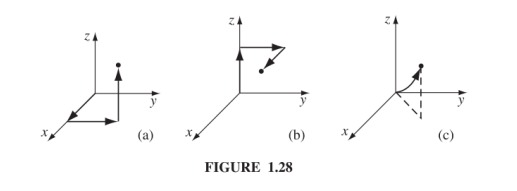
\includegraphics[width=0.7\textwidth]{1.28.jpg} 
    \label{fig:mi_figura}
\end{figure}


\textbf{Teorema Fundamental:}

\[
\int_a^b \nabla T \cdot d\mathbf{l} = T(b) - T(a)
\]

Se tiene:

\[
T(b) = 7
\]

\[
T(a) = 0 \quad \Rightarrow \quad T(0,0,0) = 0
\]

\[
\boxed{T(b) - T(a) = 7}
\]

Se calcula el gradiente de \( T \):

\[
\nabla T = \left( \frac{\partial}{\partial x} \hat{x} + \frac{\partial}{\partial y} \hat{y} + \frac{\partial}{\partial z} \hat{z} \right) (x^2 + 4xy + 2y z^3)
\]

\[
\nabla T = (2x + 4y) \hat{x} + (4x + 2z^3) \hat{y} + (6y z^2) \hat{z}
\]

Por otro lado:

\[
d\mathbf{l} = dx \hat{x} + dy \hat{y} + dz \hat{z}
\]
\[
\nabla T \cdot d\mathbf{l} = (2x + 4y)dx + (4x + 2z^3)dy + (6y z^2)dz
\]

\subsection*{Para la Primera Ruta (a):}

\textbf{En 1°:} \( x: 0 \to 1 \)

\[
y = 0, \quad z = 0
\]

\[
dy = 0, \quad dz = 0
\]

\[
\int \nabla T \cdot d\mathbf{l} = \int_0^1 2x \, dx = 2 \int_0^1 x \, dx
\]

\[
= 2 \left[ \frac{x^2}{2} \right]_0^1
\]

\[
= 2 \left( \frac{1}{2} \right) = 1
\]

\textbf{En 2°:} \( y: 0 \to 1 \)

\[
x = 1, \quad z = 0
\]

\[
dx = 0, \quad dy = 1
\]

\[
\int \nabla T \cdot d\mathbf{l} = \int_0^1 4 dy = 4 \int_0^1 dy
\]

\[
= 4 \left[ y \right]_0^1 = 4
\]

\textbf{En 3°:} \( z: 0 \to 1 \)

\[
y = 1, \quad x = 1
\]

\[
dx = 0, \quad dy = 0
\]

\[
\int \nabla T \cdot d\mathbf{l} = \int_0^1 6z^2 dz = 6 \int_0^1 z^2 dz
\]

\[
= 6 \left[ \frac{z^3}{3} \right]_0^1 = 6 \times \frac{1}{3} = 2
\]

\[
\int_a^b \nabla T \cdot d\mathbf{l} = 1 + 4 + 2 = \boxed{7}
\]


\subsection*{Para la Segunda Ruta (b):}

\textbf{En 1°:} \( z: 0 \to 1 \)

\[
y = 0, \quad x = 0
\]

\[
dx = 0, \quad dy = 0
\]

\[
\int \nabla T \cdot d\mathbf{l} = 0
\]

\textbf{En 2°:} \( y: 0 \to 1 \)

\[
x = 0, \quad z = 1
\]

\[
dx = 0, \quad dz = 0
\]

\[
\int \nabla T \cdot d\mathbf{l} = \int_0^1 2 \, dy = 2 \int_0^1 dy = 2
\]

\textbf{En 3°:} \( x: 0 \to 1 \)

\[
y = 1, \quad z = 1
\]

\[
dy = 0, \quad dz = 0
\]

\[
\int \nabla T \cdot d\mathbf{l} = \int_0^1 (2x + 4)dx
\]

\[
= \int_0^1 2x \, dx + \int_0^1 4 \, dx
\]

\[
= \left[ x^2 \right]_0^1 + 4 \left[ x \right]_0^1
\]

\[
= 1 + 4 = 5
\]

\[
\int_a^b \nabla T \cdot d\mathbf{l} = 0 + 2 + 5 = \boxed{7}
\]

\subsection*{Para la Ruta 3: \( z = x^2, \quad y = x \)}

\[
x: 0 \to 1
\]

\[
y = x, \quad z = x^2
\]

\[
dy = dx, \quad dz = 2x \, dx
\]

\[
\nabla T \cdot d\mathbf{l} = (2x + 4x)dx + (4x + 2(x^2)^3)dx + (6x(x^2)^2)2x dx
\]

\[
= (2x + 4x)dx + (4x + 2x^6)dx + 12x^6 dx
\]

\[
= (10x + 14x^6)dx
\]

\[
\int_a^b \nabla T \cdot d\mathbf{l} = \int_0^1 10x \, dx + \int_0^1 14x^6 \, dx
\]

\[
= 5 + 2 = \boxed{7}
\]

\question{Problema  1.34}
Verificación del Teorema de Stokes para la fución 
\[
\mathbf{V} = (xy) \hat{\mathbf{x}} + (2yz) \hat{\mathbf{y}} + (3zx) \hat{\mathbf{z}}
\] Usando el área triangular de la figura 1.34.
\begin{figure}[h!] 
    \centering
    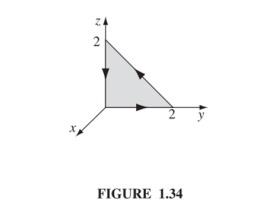
\includegraphics[width=0.5\textwidth]{1.34.jpg} 
    \label{fig:mi_figura}
\end{figure}


Teorema de Stokes
\[
\oint_{\partial S} \mathbf{V} \cdot d\mathbf{l} = \iint_{S} (\nabla \times \mathbf{V}) \cdot d\mathbf{a}
\]

Cálculo del rotacional

\[
\nabla \times \mathbf{V} =
\begin{vmatrix}
\hat{\mathbf{x}} & \hat{\mathbf{y}} & \hat{\mathbf{z}} \\
\frac{\partial}{\partial x} & \frac{\partial}{\partial y} & \frac{\partial}{\partial z} \\
xy & 2yz & 3zx
\end{vmatrix}
\]

\[
= (0 - 2y) \hat{\mathbf{x}} - (3x - 0) \hat{\mathbf{y}} + (0 - x) \hat{\mathbf{z}}
\]

\[
= -2y \hat{\mathbf{x}} - 3x \hat{\mathbf{y}} - x \hat{\mathbf{z}}
\]

Área diferencial:

\[
d\mathbf{a} = dy dz \, \hat{\mathbf{x}}
\]

\[
(\nabla \times \mathbf{V}) \cdot d\mathbf{a} = (-2y) dy dz
\]

Por tanto:

\[
\iint_S -2y \, dy dz
\]

\[
\int_2^0 \int_2^{2+z} -2y \, dy dz
\]

Para los límites de \( y \):

\[
m = \frac{z_2 - z_1}{y_2 - y_1} = \frac{2 - 0}{0 - 2} = -1
\]
\[
 z- z_1=m({y - y_1} )
\]
\[
z - 0 = m(y - 2)
\]

\[
z - 0 = -1(y - 2)
\]

\[
z = -1y + 2
\]

\[
y = 2 - z
\]

Resolviendo la integral:
\begin{align*}
    \int_0^2 dz \int_0^{2-z} (-2y) dy &= \int_0^2 dz \left[ -y^2 \right]_0^{2-z} \\
    &= \int_0^2 dz \left( - (2-z)^2 \right) \\
    &= \int_0^2 dz (-4 + 4z - z^2) \\
    &= \left[ -4z + 2z^2 - \frac{z^3}{3} \right]_0^2 \\
    &= \left( -8 + 8 - \frac{8}{3} \right) \\
    &=\boxed{ -\frac{8}{3}}
\end{align*}
Por otro lado:
\[
\oint_{\partial S} \mathbf{V} \cdot d\mathbf{l} 
\] 
La parametrización de la curva se realiza dividiéndola en tres segmentos:
\[
\lambda = \lambda_1 + \lambda_2 + \lambda_3
\]


Para el segmento en la dirección de $\hat{y}$, se tiene:

\[
y: 0 \to 1
\]

Dado que $dx = dz = 0$, entonces la integral en este tramo es:

\[
\int = 0
\]

Para el siguiente segmento, con $x = 0$:

\[
dx = 0
\]
\[
y = 2 - z
\]
\[
dy = -dz
\]

Evaluado la integral:

\[
\int 2 yz \, dy
\]

Reescribiendo la integral en términos de $z$:

\[
-\int_0^2 2(2 - z)z \, dz
\]

Desarrollando:

\[
-\int_0^2 (4z - 2z^2) \, dz
\]

\[
-\left[ \frac{4z^2}{2} - \frac{2z^3}{3} \right]_0^2
\]

\[
=-\left[ \frac{8}{2} - \frac{16}{3} \right]
\]

\[
=-\left( \frac{24 - 16}{3} \right)
\]

\[
\boxed{ =-\frac{8}{3}}
\]
\question{Problema  1.36} Demuestre que:

a) 
\[
\int_S f (\nabla \times A) \cdot da = \int_S [ A \times (\nabla f)] \cdot da + \oint_p f A \cdot dl
\]

b) 
\[
\int_V b \cdot (\nabla \times A) d\tau = \int_V A \cdot (\nabla \times B) d\tau + \int_S (A \times B) \cdot da
\]

\textbf{Solución a)}

Usando la identidad

\[
\nabla \times (f A) = f (\nabla \times A) + (\nabla f) \times A
\]

Usando Stokes:

\[
\int_S \nabla \times (f A) \cdot da = \oint_p f A \cdot dl
\]

\[
\int_S [ f (\nabla \times A) + (\nabla f) \times A ] \cdot da = \oint_p f A \cdot dl
\]

Separando la integral:

\[
\int_S f (\nabla \times A) \cdot da + \int_S [ (\nabla f) \times A ] \cdot da = \oint_p f A \cdot dl
\]

Organizando:

\[
\int_S f (\nabla \times A) \cdot da = \int_S [ A \times (\nabla f)] \cdot da + \oint_p f A \cdot dl
\]

\textbf{Solución b)}
Usando la identidad:

\[
\nabla \cdot ( A \times B ) = B \cdot (\nabla \times A) - A \cdot (\nabla \times B)
\]

Teorema de la divergencia:
\[
\int_V \nabla \cdot (A \times B) d\tau = \int_S (A \times B) \cdot da
\]

\[
\int_V \left[ B \cdot (\nabla \times A) - A \cdot (\nabla \times B) \right] d\tau = \int_S (A \times B) \cdot da
\]

\[
\int_V B \cdot (\nabla \times A) d\tau - \int_V A \cdot (\nabla \times B) d\tau = \int_S (A \times B) \cdot da
\]

Reorganizo:

\[
\int_V B \cdot (\nabla \times A) d\tau = \int_V A \cdot (\nabla \times B) d\tau + \int_S (A \times B) \cdot da
\]
\question{Problema  1.38} Exprese los vectores unitarios \( \hat{r}, \hat{\theta}, \hat{\varphi} \) en términos de \( \hat{x}, \hat{y}, \hat{z} \) y después deduzca la ec. 1.64.  Verifíque la respuesta de varias maneras (r̂⋅r̂ = 1, r̂⋅ θ̂ = 0, r̂⋅φ̂ = 0, etc.). También encontrar las fórmulas inversas, dando \( \hat{x}, \hat{y}, \hat{z} \) en términos de \( \hat{r}, \hat{\theta}, \hat{\varphi} \).

\[
r = x \hat{x} + y \hat{y} + z \hat{z}
\]

\[
x = r \sin\theta \cos\varphi
\]

\[
y = r \sin\theta \sin\varphi
\]

\[
z = r \cos\theta
\]

\[
\hat{r} = r\sin\theta \cos\varphi \hat{x} + r\sin\theta \sin\varphi \hat{y} + r\cos\theta \hat{z}
\]

\[
\hat{r}= \frac{ \frac{\partial r}{\partial r}}
{| \frac{\partial r}{\partial r}  | }}
\]

\[
\frac{\partial r}{\partial r} = \sin\theta \cos\varphi \hat{x} + \sin\theta \sin\varphi \hat{y} + \cos\theta \hat{z}
\]

\[
\left| \frac{\partial r}{\partial r} \right| = \sqrt{\sin^2\theta \cos^2\varphi + \sin^2\theta \sin^2\varphi + \cos^2\theta} 
\]
\[
= \sqrt{1} = 1
\]

\[
\boxed{\hat{r} = \sin\theta \cos\varphi \hat{x} + \sin\theta \sin\varphi \hat{y} + \cos\theta \hat{z}}
\]

Para \( \hat{\theta} \):

\[
\hat{\theta} = \frac{\frac{dr}{d\theta}}{\left| \frac{dr}{d\theta} \right|}
\]

\[
\frac{dr}{d\theta} = r \cos\theta \cos\varphi \hat{x} + r \cos\theta \sen\varphi \hat{y} - r \sen\theta \hat{z}
\]

\[
\left| \frac{dr}{d\theta} \right| = r \sqrt{\cos^2\theta (\cos^2\varphi + \sin^2\varphi) + \sin^2\theta}
\]

\[
= r \sqrt{\cos^2\theta + \sin^2\theta} = r
\]

\[
\boxed{\hat{\theta} = \cos\theta \cos\varphi \hat{x} + \cos\theta \sin\varphi \hat{y} - \sin\theta \hat{z}}
\]


Para \( \hat{\varphi} \):

\[
\hat{\varphi} = \frac{\frac{dr}{d\varphi}}{\left| \frac{dr}{d\varphi} \right|}
\]

\[
\frac{dr}{d\varphi} = -r \sin\theta \sin\varphi \hat{x} + r \sin\theta \cos\varphi \hat{y}
\]

\[
\left| \frac{dr}{d\varphi} \right| = r \sqrt{\sin^2\theta \sin^2\varphi + \sin^2\theta \cos^2\varphi}
\]

\[
\left| \frac{dr}{d\varphi} \right|= r \sin\theta
\]
\[
\boxed{\hat{\varphi} = -\sin\varphi \hat{x} + \cos\varphi \hat{y}}
\]
\]


Comprobando la respuesta:
\[
\hat{r} \cdot \hat{r} = \sin^2\theta (\cos^2\phi + \sin^2\phi) + \cos^2\theta = \sin^2\theta + \cos^2\theta = 1 \quad \checkmark
\]
\[
\hat{\theta} \cdot \hat{\phi} = -\cos\theta \sin\phi \cos\phi + \cos\theta \sin\phi \cos\phi = 0 \quad \checkmark 
\]
Ahora, para  las fórmulas inversas, dejando \( \hat{x}, \hat{y}, \hat{z} \) en términos de \( \hat{r}, \hat{\theta}, \hat{\varphi} \).


\[
\sin\theta \hat{r} = \sin^2\theta \cos\phi \hat{x} + \sin^2\theta \sin\phi \hat{y} + \sin\theta \cos\theta \hat{z}.
\]

\[
\cos\theta \hat{\theta} = \cos^2\theta \cos\phi \hat{x} + \cos^2\theta \sin\phi \hat{y} - \sin\theta \cos\theta \hat{z}.
\]

Añadiendo estas ecuaciones:

\begin{enumerate}
    \item $\sin\theta \hat{r} + \cos\theta \hat{\theta} = +\cos\phi \hat{x} + \sin\phi \hat{y}$
    \item $\hat{\phi} = -\sin\phi \hat{x} + \cos\phi \hat{y}$
\end{enumerate}

Multiplicando (1) por $\cos\phi$, (2) por $\sin\phi$ y restando:

\[
\boxed{\hat{x} = \sin\theta \cos\phi \hat{r} + \cos\theta \cos\phi \hat{\theta} - \sin\phi \hat{\phi}.}
\]

Multiplicando (1) por $\sin\phi$, (2) por $\cos\phi$ y sumando:

\[
\boxed{\hat{y} = \sin\theta \sin\phi \hat{r} + \cos\theta \sin\phi \hat{\theta} + \cos\phi \hat{\phi}.}
\]

\[
\cos\theta \hat{r} = \cos\theta \sin\theta \cos\phi \hat{x} + \cos\theta \sin\theta \sin\phi \hat{y} + \cos^2\theta \hat{z}.
\]

\[
\sin\theta \hat{\theta} = \sin\theta \cos\theta \cos\phi \hat{x} + \sin\theta \cos\theta \sin\phi \hat{y} - \sin^2\theta \hat{z}.
\]

Restando estas ecuaciones:

\[
\boxed{\hat{z} = \cos\theta \hat{r} - \sin\theta \hat{\theta}.}
\]

\end{document}